\documentclass[12pt]{article}
\usepackage[a4paper, margin=1in]{geometry} 
\usepackage{graphicx} 
\usepackage{hyperref}
\usepackage{float}
\usepackage{multicol}
\usepackage{amsmath}
\usepackage[ruled]{algorithm2e}
\usepackage{amssymb}
\usepackage[font=small, labelfont=bf]{caption}

\title{Lecture Notes for \\ INF281 Basics of Bioinformatics Sequence Analysis}
\author{Takaya Saito}
\date{}

\begin{document}

\pagenumbering{arabic}
\setcounter{page}{8}

\makeatletter 
\renewcommand{\thefigure}{\arabic{section}.\arabic{figure}}
\renewcommand{\thetable}{\arabic{section}.\arabic{table}}
\makeatother

%
% PART II
%
\setcounter{part}{1}
\part{}

%
% Global_pairwise_alignment
%
\setcounter{section}{1}
\setcounter{figure}{0}
\setcounter{table}{0}
\section{Global pairwise alignment}
%\documentclass[12pt]{article}
%\usepackage[a4paper, margin=1in]{geometry} 
%\usepackage{graphicx} 
%\usepackage{hyperref}
%\usepackage{float}
%\usepackage{multicol}
%\usepackage[font=small, labelfont=bf]{caption}
%
%\begin{document}

%
% Pairwise alignment
%
\subsection{Pairwise alignment}
A pairwise alignments is a basic sequence structure that consits of two sequences. A global alignment stretches to the whole part of two sequences, whereas a local alignment usually contains only part of the sequences.

%
% Pairwise alignment
%
\subsubsection*{Components of pairwise alignment}

We name two sequences as ‘database’ or ‘d’ and ‘query’ or ‘q’ through this course. They may represent sequences from two different species or organisms.
\\

\noindent
Identical sequences.
\begin{verbatim}
    q: ACGT
    d: ACGT
\end{verbatim}

\noindent
One mismatch.
\begin{verbatim}
    q: ACGT
    d: ACGA
\end{verbatim}

\noindent
The '-' symbol represents a blank. A single or a set of multile blanks further reprents a gap, which is an indication of insertion or deletion in the course of evoluation between two organisms.
\begin{verbatim}
    q: ACGT
    d: A-GT
\end{verbatim}

\noindent
\textbf{N.B.} A gap cannot be aligned with another gap.

%
% Example of a simple scoring scheme
%
\subsubsection*{Example of a simple scoring scheme}
\begin{itemize}
\item Match: 1
\item Mismatch: 0
\item Gap penalty: 1 (use -1 for the actual calculation)
\end{itemize}

\noindent
We may use the following notation.
\begin{itemize}
\item $R_{ab}$ = 1 for a = b
\item $R_{ab}$ = 0 for a $\neq$ b
\item g = 1
\end{itemize}

%
% NEW PAGE
%
\newpage 

%
% Exercise \thesection.1
%
\subsubsection*{Exercise \thesection.1}
Use the simple scoring scheme above and calculate the scores of the following two alignments.

\begin{multicols}{2}
\begin{verbatim}
Alignment 1
    q: GCA-GCA
    d: GA-TG-A	
\end{verbatim}

\begin{verbatim}
Alignment 2 
    q: GCA-GCA
    d: GA-TG-A	
\end{verbatim}
\end{multicols}

%\end{document}

%\documentclass[12pt]{article}
%\usepackage[a4paper, margin=1in]{geometry} 
%\usepackage{graphicx} 
%\usepackage{hyperref}
%\usepackage{float}
%\usepackage{multicol}
%\usepackage[font=small, labelfont=bf]{caption}
%
%\begin{document}

%
% Alignment by brute-force
%
\subsection{Alignment by brute--force}
A brute--force approach finds the alignment with the highest score by simply considering all possible alignments and calculates the score for each of them.

%
% An example of brute--force approach
%
\subsubsection*{An example of brute--force approach}
We find the optimal alignment for the following sequences by using the scoring scheme below.

\begin{multicols}{2}
Sequences:
\begin{verbatim}
    q: AG, d: ACG
\end{verbatim}
\vfill\null
\columnbreak

\noindent Scoring scheme: \\ 
\null \quad $R_{ab}$ = 1 for a = b \\ 
\null \quad $R_{ab}$ = 0 for a $\neq$ b \\ 
\null \quad g = 1

\end{multicols} 

\noindent \textbf{1. The length of alignment}
\begin{itemize}
\item Maximum length: length(q) + length(d)
\item Minimum length: max(length(q), length(d))
\end{itemize}
\medskip 

\noindent \textbf{2. All possible alignments when length = 5}
\begin{verbatim}
    ---AG    A---G    A--G-    AG---    --A-G
    ACG--    -ACG-    -AC-G    --ACG    AC-G-

    --AG-    -AG--    -A--G    -A-G-    A-G--
    AC--G    A--CG    A-CG-    A-C-G    -A-CG
\end{verbatim}
\medskip

\noindent \textbf{3. All possible alignments when length = 4}
\begin{verbatim}
    A--G    A-G-    AG--    A--G    -A-G    -AG-
    ACG-    AC-G    A-CG    -ACG    ACG-    AC-G

    -AG-    A-G-    --AG    --AG    -A-G    AG--
    A-CG    -ACG    ACG-    AC-G    A-CG    -ACG
\end{verbatim}
\medskip

\noindent \textbf{4. All possible alignments when length = 3}
\begin{verbatim}
    -AG    A-G    AG-
    ACG    ACG    ACG
\end{verbatim}
\medskip

\noindent \textbf{5. Alignment with the best score}
\begin{verbatim}
    ACG
    A-G	
\end{verbatim}

Score: 1

%
% Search space size of the brute-force approach
%
\subsubsection*{Search space size of the brute-force approach}
The search space size is the number of all possible alignments. It is 25 (10 + 12 + 3) for the example above. \\

\noindent \textbf{Rapid growth of search space size}

\begin{multicols}{2}
\begin{verbatim}
Example 1
    q: ACGACG, d: AGAG
\end{verbatim}
Search space size: 1289

\begin{verbatim}
Example 2
    q: ACGACGACGACG, d: AGAGAGAG
\end{verbatim}
Search space size: 4,673,345

\end{multicols}

%
% Exercise \thesection.2
%
\subsubsection*{Exercise \thesection.2}
Find the alignment with the best score for the sequences.  Use the simple scoring scheme below.

\begin{multicols}{2}
Sequences:
\begin{verbatim}
    q: A, d: AC
\end{verbatim}
\vfill\null
\columnbreak

\noindent Scoring scheme: \\ 
\null \quad $R_{ab}$ = 1 for a = b \\ 
\null \quad $R_{ab}$ = 0 for a $\neq$ b \\ 
\null \quad g = 1

\end{multicols} 

\begin{enumerate}
\item What are the maximum and minimum lengths of the alignment?
\item Identify all possible alignments.
\item What is the best score?
\item What is the search space size when the brute-force approach is used?
\end{enumerate}

%\end{document}

%\documentclass[12pt]{article}
%\usepackage[a4paper, margin=1in]{geometry} 
%\usepackage{graphicx} 
%\usepackage{hyperref}
%\usepackage{float}
%\usepackage{multicol}
%\usepackage[font=small, labelfont=bf]{caption}
%
%\begin{document}

%
% Alignment by brute-force
%
\subsection{Table representation of alignment}
Several data strcutres can be used to repesent an alignment. The table representation is frequently used and also makes the process clear when we combine it with dynamic programming (DP) later.

\subsubsection*{Data structures and algorithms}
It is important to consider the following aspects before solving computational problems.
\begin{enumerate}
\item Identify and analyze the problem you want to solve
\item Pick up an algorithm that can efficiently solve the problem
\item Decide a data structure that works with the algorithm of your choice
\end{enumerate}

\noindent We use a table format (2D array) to solve global alignments by dynamic programming.

\subsubsection*{Example of table format}
Alignment:
\begin{verbatim}
    q: -AG-
    d: A-CG
\end{verbatim}
\medskip 

\noindent \textbf{1. Initial setup}

\begin{enumerate}
\item Make a table with the size of (1 + length(q)) by (1 + length(b))
\item Add the database sequence as column labels
\item And the query sequence as row labels
\end{enumerate}

\begin{figure}[H]
  \centering
      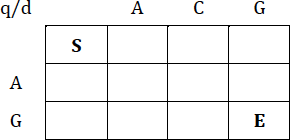
\includegraphics[width=0.3\textwidth]{fig02/alignment_to_table.png}
\end{figure}

\noindent \textbf{2. Add arrows}

We use three types of arrows to form an alignment.
\begin{itemize}
\item Move diagonally: add the letters from ‘q’ and ‘d’ to the alignment
\item Move vertically: add ‘-’ and the letter from ‘d’ to the alignment
\item Move horizontally: add the letter from ‘q’ and ‘-’ to the alignment
\end{itemize}

It shoud start from S and stops at E.

\begin{figure}[H]
  \centering
      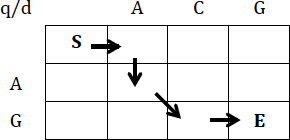
\includegraphics[width=0.3\textwidth]{fig02/alignment_to_table_example.png}
\end{figure}

%
% Exercise \thesection.3
%
\subsubsection*{Exercise \thesection.3}

Find the corresponding alignments for Table 1, 2 and 3.

\begin{multicols}{3}
Table 1
\begin{figure}[H]
  \centering
      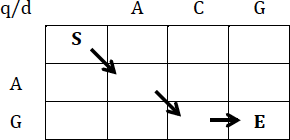
\includegraphics[width=0.3\textwidth]{fig02/alignment_to_table_exercise1.png}
\end{figure}

Table 2
\begin{figure}[H]
  \centering
      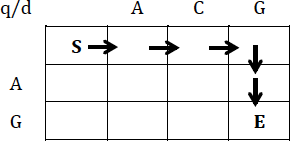
\includegraphics[width=0.3\textwidth]{fig02/alignment_to_table_exercise2.png}
\end{figure}

Table 3
\begin{figure}[H]
  \centering
      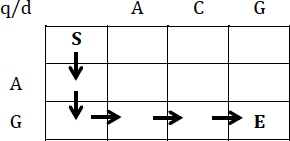
\includegraphics[width=0.3\textwidth]{fig02/alignment_to_table_exercise3.png}
\end{figure}

\end{multicols} 

%\end{document}

%\documentclass[12pt]{article}
%\usepackage[a4paper, margin=1in]{geometry} 
%\usepackage{graphicx} 
%\usepackage{hyperref}
%\usepackage{float}
%\usepackage{multicol}
%\usepackage{amsmath}
%\usepackage[ruled]{algorithm2e}
%\usepackage[font=small, labelfont=bf]{caption}
%
%\begin{document}

%
% Global alignment with DP
%
\subsection{Global alignment with DP}
Dynamic programming (DP) provides a solution for a multi-stage decision process, in which larger decisions recursively nest smaller decisions.

\subsubsection*{Memorize the best score in a table cell}

The most basic step of DP procedures is updatig a cell with the hightet score from the three different scores calculated from its adjacent cells. DP ends when all the table cells are updated.

\begin{figure}[H]
  \centering
      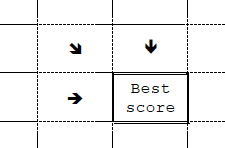
\includegraphics[width=0.25\textwidth]{fig02/dynamic_programmoing_cell_update.png}
\end{figure}

%
% Table notation and indices
%	
\subsubsection*{Table notation and indices}
$H_{i,j}$ represents the score of the cell for the current update. $H_{i-1,j}$, $H_{i,j-1}$,and $H_{i-1,j-1}$ are the scores of the adjacent cells.

\begin{multicols}{2}

Cell $H_{i, j}$ and its adjcent cells
\begin{figure}[H]
  \centering
      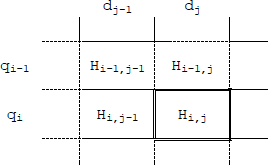
\includegraphics[width=0.3\textwidth]{fig02/dynamic_programmoing_cell_indices.png}
\end{figure}

Example
\begin{figure}[H]
  \centering
      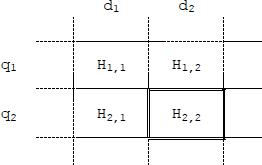
\includegraphics[width=0.3\textwidth]{fig02/dynamic_programmoing_cell_indices_example.png}
\end{figure}

\end{multicols} 

%
% Calculation of three candidate scores
%	
\subsubsection*{Calculation of three candidate scores}
$H_{i,j}^{(0)}$, $H_{i,j}^{(1)}$, and $H_{i,j}^{(2)}$ represent the three candidate scores of $H_{i,j}$. They are respectively calculated as:
\begin{align*}
H_{i,j}^{(0)} &= H_{i-1,j} - g &(vertical) \\
H_{i,j}^{(1)} &= H_{i,j-1} - g	&(horizontal) \\
H_{i,j}^{(2)} &= H_{i-1,j-1} + R_{a,b} &(diagonal)
\end{align*}

%
% Exercise \thesection.4
%
\subsubsection*{Exercise \thesection.4}

Calculate the scores of $H_{4,6}^{(0)}$, $H_{4,6}^{(1)}$, and $H_{4,6}^{(2)}$ first and then update $H_{4,6}$.
\begin{multicols}{2}
\begin{figure}[H]
  \centering
      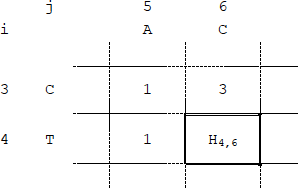
\includegraphics[width=0.3\textwidth]{fig02/dynamic_programmoing_cell_update_exercise.png}
\end{figure}

\noindent Scoring scheme: \\ 
$R_{ab}$ = 1 for a = b \\ 
$R_{ab}$ = 0 for a $\neq$ b \\ 
g = 1

\end{multicols} 

%
% Initialization
%
\subsubsection*{Initialization}

The first row and the first column can be calcuated independently from the adjcent cells.
\begin{align*}
H_{0,j} &:  j * -1 * g \\
H_{i,0} &: i * -1 * g
\end{align*}

\noindent
Example
\begin{figure}[H]
  \centering
      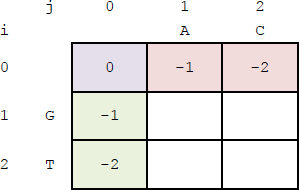
\includegraphics[width=0.3\textwidth]{fig02/dynamic_programmoing_initialization.png}
\end{figure}

%
% Exercise \thesection.5
%
\subsubsection*{Exercise \thesection.5}
Update all cells of Table 1 and 2. Use the scoring scheme in Exercise \thesection.4.

\begin{multicols}{2}
Table 1
\begin{figure}[H]
  \centering
      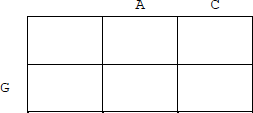
\includegraphics[width=0.3\textwidth]{fig02/global_alignment_exercise1.png}
\end{figure}

\vfill\null
\columnbreak

Table 2
\begin{figure}[H]
  \centering
      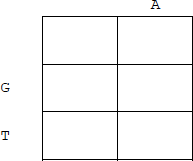
\includegraphics[width=0.25\textwidth]{fig02/global_alignment_exercise2.png}
\end{figure}

\end{multicols} 

%
% Sub-solutions
%
\subsubsection*{Sub-solutions}

In DP, larger decisions recursively nest smaller decisions. For instance, Table S is included in Table L.

\begin{multicols}{2}
Table S
\begin{figure}[H]
  \centering
      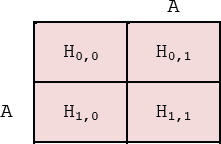
\includegraphics[width=0.3\textwidth]{fig02/dynamic_programmoing_subsolution_S.png}
\end{figure}

\vfill\null
\columnbreak

Table L
\begin{figure}[H]
  \centering
      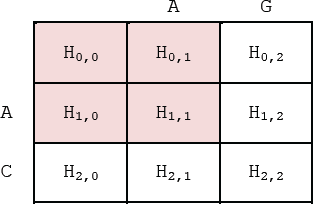
\includegraphics[width=0.4\textwidth]{fig02/dynamic_programmoing_subsolution_L.png}
\end{figure}

\end{multicols} 

%
% NEW PAGE
%
\newpage

%
% Psedo-code of global alignment with DP
%
\subsubsection*{Psedo-code of updating DP table for global alignment}

\begin{algorithm}[H]
  \SetKwInOut{HAB}{$\mathrm{H_{i,j}}$}
  \SetKwInOut{RAB}{$\mathrm{R_{a,b}}$}
  \SetKwInOut{G}{$\mathrm{g}$}
  \SetKwData{dRAB}{$\mathrm{R_{a,b}}$}
  \SetKwData{dG}{$\mathrm{g}$}
  
  \BlankLine
    
  \HAB{Dyanamic programming table}
  \RAB{Match/mismatch scores}
  \G{Gap penalty}
  
  \BlankLine \BlankLine
  
  \tcp{Initialization}
  \For{$i \leftarrow 0$ \KwTo $m$}{
    $\mathrm{H_{i,0}}$ $\leftarrow$ $i * -1 * g$\;
  }
  \For{$j \leftarrow 1$ \KwTo $n$}{
    $\mathrm{H_{0,j}}$ $\leftarrow$ $j * - 1 * g$\;
  }
  
  \BlankLine \BlankLine
    
  \tcp{Main loop for table update}
  \For{$i \leftarrow 1$ \KwTo $m$}{
    \For{$j \leftarrow 1$ \KwTo $n$}{
      $\mathrm{H_{i,j}}$ $\leftarrow$ $max(\mathrm{H_{i-1,j}} - \dG, \mathrm{H_{i,j-1}} - \dG, \mathrm{H_{i-1,j-1}}$ + \dRAB)\;
    }
  }
  
  \SetAlgoRefName{\thesection.1}
  \caption{Update dynamic programming table for global alignment}

\end{algorithm}

%\end{document}

%\documentclass[12pt]{article}
%\usepackage[a4paper, margin=1in]{geometry} 
%\usepackage{graphicx} 
%\usepackage{hyperref}
%\usepackage{float}
%\usepackage{multicol}
%\usepackage{amsmath}
%\usepackage[ruled]{algorithm2e}
%\usepackage{amssymb}
%\usepackage[font=small, labelfont=bf]{caption}

%\begin{document}

%
% Backtracking
%
\subsection{Backtracking}
Backtracking is a post-processing procedure to find the alignments that have yielded the best score. 

%
% Store movement in cells
%
\subsubsection*{Store movement in cells}

A table cell can be used for storing the movement.
\begin{figure}[H]
  \centering
      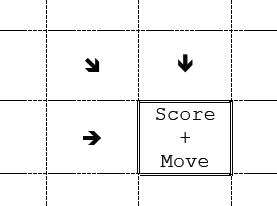
\includegraphics[width=0.3\textwidth]{fig02/back_tracking_store_moves.png}
\end{figure}

\noindent \textbf{Example}
\begin{multicols}{2}
Cells with scores and directions
\begin{figure}[H]
  \centering
      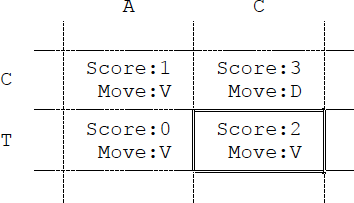
\includegraphics[width=0.3\textwidth]{fig02/back_tracking_store_moves_example.png}
\end{figure}

Use arrows to indicate backtracking
\begin{figure}[H]
  \centering
      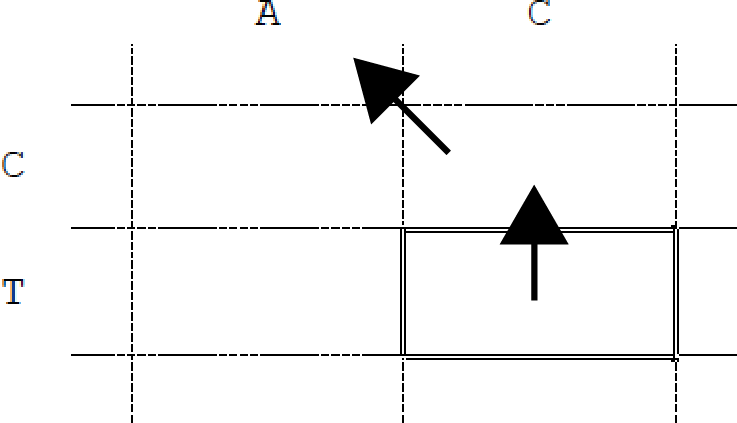
\includegraphics[width=0.3\textwidth]{fig02/back_tracking_store_moves_arrows.png}
\end{figure}

\end{multicols} 

%
% Exercise \thesection.6
%
\subsubsection*{Exercise \thesection.6}
	
Complete the DP table with scores and directions. What is the alignment with the best score?

\begin{multicols}{2}
\begin{figure}[H]
  \centering
      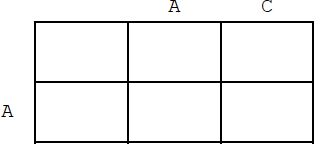
\includegraphics[width=0.3\textwidth]{fig02/back_tracking_store_moves_exercise.png}
\end{figure}

\noindent Scoring scheme: \\ 
$R_{ab}$ = 1 for a = b \\ 
$R_{ab}$ = 0 for a $\neq$ b \\ 
g = 1

\end{multicols} 

%
% Re-calculate candidate scores
%
\subsubsection*{Re-calculate candidate scores}

Re-calculating the three candidate scores also reveals the movement.

\begin{align*}
H_{i,j}^{(0)} &= H_{i-1,j} - g &(vertical) \\
H_{i,j}^{(1)} &= H_{i,j-1} - g &(horizontal) \\
H_{i,j}^{(2)} &= H_{i-1,j-1} + R_{a,b} &(diagonal)
\end{align*}

\noindent \textbf{Example}

\begin{figure}[H]
  \centering
      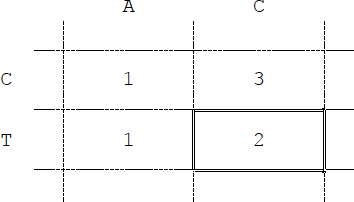
\includegraphics[width=0.3\textwidth]{fig02/back_tracking_example.png}
\end{figure}
				
\begin{align*}
H_{i,j}^{(0)} &= 3 - 1 = 2 = H_{i,j} &\checkmark & (vertical) \\
H_{i,j}^{(1)} &= 1 - 1 = 0 \neq H_{i,j} &\hfill & (horizontal) \\
H_{i,j}^{(2)} &= 1 + 0 = 1 \neq H_{i,j} &\hfill  & (diagonal)
\end{align*}

%
% Common mistake with backtracking
%
\subsubsection*{Common mistake with backtracking}
For the re-calculation approach, it is not to find $max(H_{i-1,j}, H_{i,j-1}, H_{i-1,j-1})$. You must re-calculate the candidates and then $max(H_{i,j}^{(0)}, H_{i,j}^{(1)} , H_{i,j}^{(2)})$ to find the actual direction.

%
% Implementation with recursive call
%
\subsubsection*{Implementation with recursive call}
Recursive calls are usually used to implement DP backtracking.

\begin{algorithm}[H]
  \SetKwInOut{HAB}{$\mathrm{H_{i,j}}$}
  \SetKwInOut{RAB}{$\mathrm{R_{a,b}}$}
  \SetKwInOut{G}{$\mathrm{g}$}
  
  \SetKwProg{Fn}{proc}{}{end}
  \SetKwInOut{I}{$\mathrm{i}$}
  \SetKwInOut{J}{$\mathrm{j}$}
  \SetKwInOut{SQ}{$\mathrm{S_{q}}$}
  \SetKwInOut{SD}{$\mathrm{S_{d}}$}
  \SetKwInOut{AQ}{$\mathrm{A_{q}}$}
  \SetKwInOut{AD}{$\mathrm{A_{d}}$}
  \SetKwInOut{K}{$\mathrm{k}$}

  \SetKwData{dI}{$\mathrm{i}$}
  \SetKwData{dJ}{$\mathrm{j}$}
  \SetKwData{dAQ}{$\mathrm{A_{q}}$}
  \SetKwData{dAD}{$\mathrm{A_{d}}$}
  \SetKwData{dK}{$\mathrm{k}$}
    
  \SetKwData{dRAB}{$\mathrm{R_{a,b}}$}
  \SetKwData{dG}{$\mathrm{g}$}

  \BlankLine
  
  \SQ{Sequence q}
  \SD{Sequence d}     
  \HAB{Dynamic programming table}
  \RAB{Match/mismatch scores}
  \G{Gap penalty}

  \BlankLine \BlankLine

  \Fn{backTrack(\dI, \dJ, \dAQ, \dAD, \dK)}{
    
    \BlankLine
    
    \I{Index of sequence q}
    \J{Index of sequence d}
    \AQ{q part of alignment (stored in reverse order)}
    \AD{d part of alignment (stored in reverse order)}
    \K{Index for \dAQ and \dAD}
  
    \BlankLine
    
    \tcp{}
    \tcp{Need to implement recursion termination here}
    \tcp{...}
    \tcp{}
        
    \BlankLine
    
    \If(\tcp*[f]{vertical}){$\mathrm{H_{i,j}} = \mathrm{H_{i-1,j}} - g$}{
      $\mathrm{A_{q, k}} $ $\leftarrow$ $ S_{q, i}$\;
      $\mathrm{A_{d, k}} $ $\leftarrow$ $ $ '-'\;
      $backTrack$($\mathrm{i-1}$, \dJ, \dAQ, \dAD, $k + 1$)\;
    }
    \BlankLine

    \If(\tcp*[f]{horizontal}){$\mathrm{H_{i,j}} = \mathrm{H_{i,j-1}} - g$}{
      $\mathrm{A_{q, k}} $ $\leftarrow$ '-'\;
      $\mathrm{A_{d, k}} $ $\leftarrow$ $ S_{d, i}$\;
      $backTrack$(\dI, $\mathrm{j-1}$, \dAQ, \dAD, $k + 1$)\;
    }
    \BlankLine
    
    \If(\tcp*[f]{diagonal}){$\mathrm{H_{i,j}} = \mathrm{H_{i-1,j-1}} +\mathrm{R_{S_{q, i},S_{d, i}}}$}{
      $\mathrm{A_{q, k}} $ $\leftarrow$ $ S_{q, i}$\;
      $\mathrm{A_{d, k}} $ $\leftarrow$ $ S_{d, i}$\;
      $backTrack$($\mathrm{i-1}$, $\mathrm{j-1}$, \dAQ, \dAD, $k + 1$)\;
    }
      
    \BlankLine
  }

  \SetAlgoRefName{\thesection.2}
  \caption{DP backtracking}

\end{algorithm}

%
% Exercise \thesection.7
%
\subsubsection*{Exercise \thesection.7}
	
Find the alignment with the best score.

\begin{multicols}{2}
\begin{figure}[H]
  \centering
      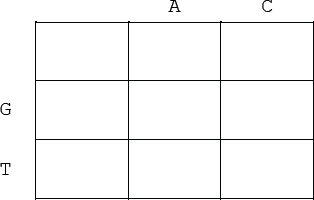
\includegraphics[width=0.3\textwidth]{fig02/back_tracking_exercise.png}
\end{figure}

\noindent Scoring scheme: \\ 
$R_{ab}$ = 1 for a = b \\ 
$R_{ab}$ = 0 for a $\neq$ b \\ 
g = 1

\end{multicols} 

%\end{document}

%\documentclass[12pt]{article}
%\usepackage[a4paper, margin=1in]{geometry} 
%\usepackage{graphicx} 
%\usepackage{hyperref}
%\usepackage{float}
%\usepackage{multicol}
%\usepackage{amsmath}
%\usepackage[ruled]{algorithm2e}
%\usepackage{amssymb}
%\usepackage[font=small, labelfont=bf]{caption}
%
%\begin{document}

%
% Needleman-Wunsch
%
\subsection{Needleman-Wunsch algorithm}
The method of using DP to solve global pairwise alignment is called the Needleman-Wunsch algorithm in the field of bioinformatics. 

%
% Complexity
%
\subsubsection*{Complexity}
\begin{itemize}
\item Time: O(nm)
\item Space: O(nm)
\end{itemize}

%
% Comparisons with other algorithms
%
\subsubsection*{Comparisons with other algorithms}
The Needleman-Wunsch algorithm is similar to several algorithms.
\\

\noindent
\textbf{Divide and conquer algorithms}

\noindent
Sub-solutions must be independent with divide and conquer.

\begin{figure}[H]
  \centering
      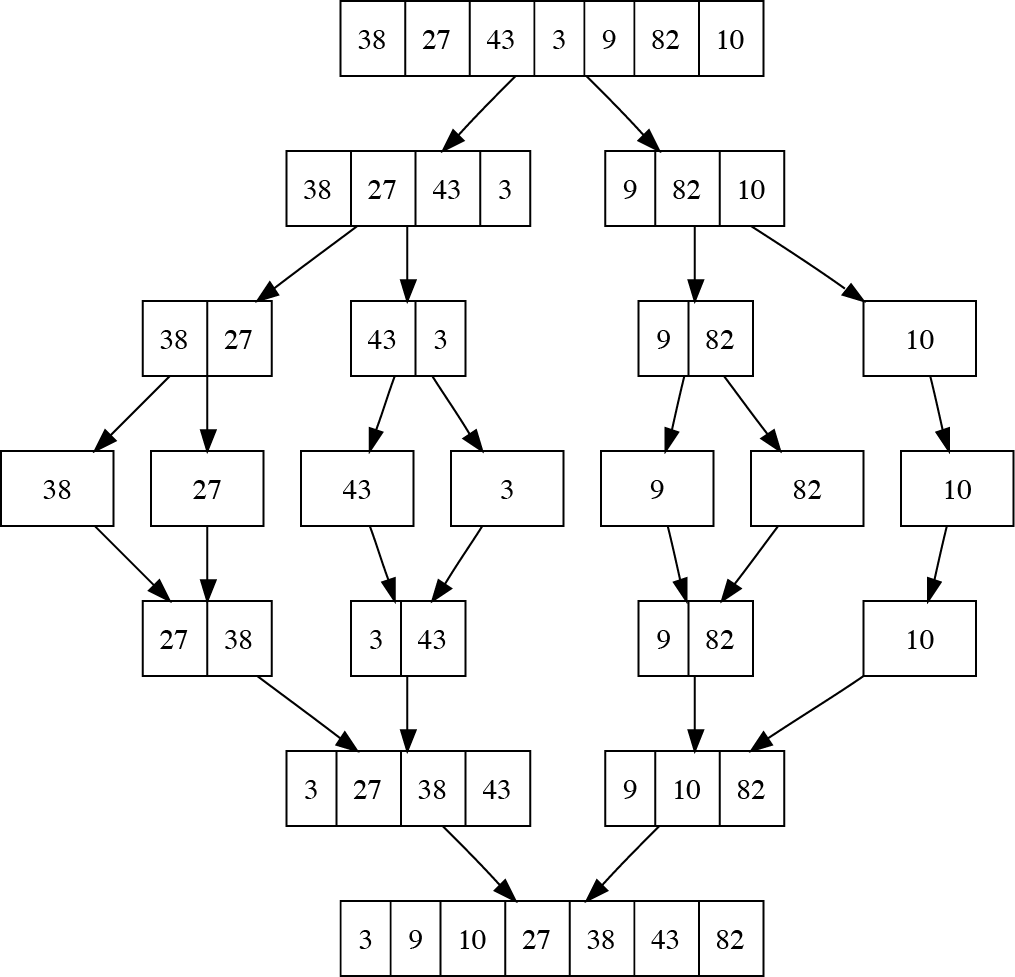
\includegraphics[width=0.25\textwidth]{fig02/Merge_sort_algorithm.png}
  \caption{Merge sort (source: \href{https://commons.wikimedia.org/w/index.php?curid=8004317}{VineetKumar, Wikimedia Commons})}
\end{figure}

\noindent
\textbf{Dijkstra's algorithm}

\noindent
Worst-case performance of Dijkstra: $O(|E|+|V|\log |V|)$

\begin{figure}[H]
  \centering
      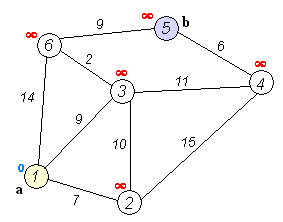
\includegraphics[width=0.25\textwidth]{fig02/Dijkstra.png}
  \caption{Dijkstra's algorithm (source: \href{https://commons.wikimedia.org/w/index.php?curid=6282617}{Ibmua, Wikimedia Commons})}
\end{figure}

%\end{document}


\end{document}
